\documentclass[11pt,a5paper]{article}

\usepackage[T1]{fontenc}
\usepackage[utf8]{inputenc}
\usepackage{lmodern, microtype}
\usepackage[estonian]{babel}
\usepackage{siunitx}
\sisetup{inter-unit-product=\ensuremath{{}\cdot{}}, per-mode=fraction, exponent-product=\cdot, output-decimal-marker={,}}
\usepackage{graphicx}
\usepackage{wrapfig}
\usepackage{adjustbox}
\usepackage{tikz}
\usetikzlibrary{arrows.meta, patterns, patterns.meta}
\usepackage{pgfplots}
\usepackage[european]{circuitikz}

\usepackage{amsmath,amssymb}
\usepackage{amsfonts}
\usepackage[hidelinks]{hyperref}
\usepackage{csquotes}
\usepackage{caption}
\usepackage{enumitem}
\topmargin=-3.0cm \textheight=19cm \textwidth=12.9cm
\oddsidemargin=-1.5cm  \evensidemargin=-1.5cm
\setlength{\parindent}{0pt} \setlength{\parskip}{6pt} \sloppy
\sloppy \relpenalty=10000 \binoppenalty=10000
\pagestyle{empty}

\newcommand{\numb}[1]{\vspace{5pt}\textbf{\large #1}}
\newcommand{\nimi}[1]{(\textsl{\small #1})}
\newcommand{\punktid}[1]{(\emph{#1~p.})}
\newcounter{ylesanne}
\newcommand{\yl}[1]{\addtocounter{ylesanne}{1}\numb{\theylesanne.} \nimi{#1} \newblock{}}
\newcommand{\autor}[1]{}% Kasuta võistluse ajal
%\newcommand{\autor}[1]{\emph{Autor: #1}}% Kasuta kui vaja autorit

\begin{document}
\begin{center}
  \textbf{\Large Eesti koolinoorte 69. füüsikaolümpiaad} \par
  \emph{12. veebruar 2021. a.\\Gümnaasiumi ülesanded (10.--12. klass)}
\end{center}

\resizebox{\textwidth}{!}{
  \emph{%
    \begin{tabular}{@{}l@{}}
      \textbf{Palun kirjutada iga ülesande lahendus eraldi lehele.}\\
      Lahendamisaeg on 5 tundi. \\
      Iga osavõtja võib lahendada kõiki pakutud ülesandeid. \\
      Arvesse lähevad 5 suurima punktide arvu saanud teoreetilist ja 1 eksperimentaalne ülesanne. \\
      Kasutada võib kirjutus- ja joonestusvahendeid ning kalkulaatorit. Muud abivahendid on keelatud.\\
      Eksperimentaalülesande lahendamisel võib kasutada üksnes loetelus toodud vahendeid. \\
      Mõõtemääramatuse hindamist ei nõuta.
    \end{tabular}
  }
} \par

\yl{PEEGEL PEEGLIS}
Toas on kaks tasapeeglit. Arvo (tähistatud punktiga $A$) nägi peeglisse vaadates Pärti (tähistatud punktiga $B$). Konstrueerige kiirte käik, kuidas Arvo võis peegli(te) abil Pärti näha. Leidke kõik võimalused. Lahendage ülesanne lisalehel.
\punktid{6} \autor{Richard Luhtaru}
\begin{figure}[h]
  \vspace{-1em}
  \centering
  \includegraphics[height=11em, trim=0 80 0 140, clip]{spiegel_joonis}
  \vspace{-2em}
\end{figure}

\yl{JUHE}
Peeter tahab vältida kasvuhoones taimede külmumist ja viib sinna elektriradiaatori nimivõimsusega $P=\qty{2}{\kW}$ ja nimipingega $V_0=\qty{230}{\V}$. Ta kasutab selleks pikendusjuhet pikkusega $L=\qty{40}{\m}$, mis  sisaldab kahte kõrvuti paiknevat vasktraati ristlõikepindalaga $S=\qty{1}{\mm\squared}$. Vase eritakistus $\rho=\qty{17}{\mohm\mm\squared\per\m}$. Milline soojuslik võimsus eraldub juhtmetes, kui tegelik võrgupinge pistikus on $V_p=\qty{240}{V}$?
\punktid{8} \autor{Jaan Kalda}

\yl{LIUMÄGI}
Liumägi koosneb kahest osast: kaldpind nurgaga $\alpha$ ja horisontaalne pind. Liumäe kõrgus on $h$ ja horisontaalne pikkus on $l$ (vt joonist). Liumägi tahetakse teha selline, et sealt alla lastes jõuaks täpselt liumäe lõppu, aga jäädes lõpus paigale. Võib eeldada, et üleminek kaldpinnalt horisontaalsele pinnale on sujuv. Milline peaks olema sellise liumäe jaoks hõõrdetegur $\mu$ liumäe ja allalaskja vahel?
\punktid{8} \autor{Kaarel Kivisalu}
\begin{figure}[h]
  \vspace{-1.5em}
  \centering
  {
    \tikzset{component/.style={draw,thick,circle,fill=white,minimum size=0.75cm,inner sep=0pt}}
    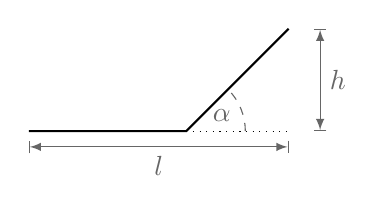
\begin{tikzpicture}
      %lines
      \draw[thick] (0,0) -- (2,0) -- (3.3,1.3);
      \draw[dotted] (2,0) -- (3.3,0);
      %angle
      \draw[dashed, black!60] (2.75,0) arc (0:45:.75);
      \draw[black!60] (2.45,0.2) node {$\alpha$};
      %lenghts
      \draw[|<->|, >=latex, black!60] (3.7,0)-- (3.7,1.3) node[midway, right]{$h$};
      \draw[|<->|, >=latex, black!60] (0,-0.2)-- (3.3,-0.2) node[midway, below]{$l$};
    \end{tikzpicture}
  }
  \vspace{-2em}
\end{figure}

\yl{KAKS TUBA}
Majas asub kaks ruudukujulist tuba, millel on üks ühine sein, ülejäänud seinad on välisseinad. Kõik seinad on identsed ja iga seina soojusjuhtivustegur on $k$. Ühes toas on lisaks tavalisele küttele lisaks kütteallikas võimsusega $P$. Kui suur on tubade temperatuurierinevus? Võib eeldada, et soojusvahetus ei toimu läbi põranda ja lae.
\\\emph{Vihje}: Soojusvahetuse võimsus läbi seina avaldub kujul $N=k(T_1-T_2)$, kus $k$ on soojusjuhtivustegur ning $T_1$ ja $T_2$ seina kahe pinna temperatuurid.
\punktid{8} \autor{Jarl Patrick Paide}

\yl{SATELLIITTELEVISIOON}
Lapimaal, laiuskraadil $\varphi =\ang{67}$ elav Jussi soovib endale paigaldada satelliittelevisiooni. Satelliittelevisiooni võimaldavad satelliidid on geostatsionaarsel orbiidil. Eeldage, et satelliittelevisioon toimib, kui satelliit asub horisondist kõrgemal. Maa raadius $R=\qty{6371}{\km}$, Maa pöörlemisperiood $T=\qty{23}{\hour}\, \qty{56}{\min}$ ja raskuskiirenus maapinnal $g= \qty{9.81}{\m\per\s\squared}$.\\
\osa Kas Jussi saab endale satelliittelevisiooni paigaldada?\\
\osa Mis on suurim laiuskraad, millel on satelliittelevisiooni paigaldamine veel võimalik?
\\ \emph{Märkus}: satelliit geostatsionaarsel orbiidil on maapinna suhtes paigal.
\punktid{8} \autor{Krister Kasemaa}

\begin{wrapfigure}{r}{2.8cm}
  \vspace{-2em}
  \begin{center}
    \includegraphics[width=2.8cm]{pall}
  \end{center}
  \vspace{-2em}
\end{wrapfigure}
\yl{DOOMINO}
Väike kuulike liigub horisontaalselt kiirusega $u$ joonisel näidatud suunas ja kukub alla kõrguselt $H$. Alumisel tasapinnal on doominoklots kõrgusega $h$, mis kukub ümber, kui kuulike sellele pihta läheb. Klotsi kaugus astmest on $d$. Leidke minimaalne algkiirus $u$, mille korral kuulike teeb ühe põrke ja lendab seejärel klotsist üle. Eeldage, et õhutakistus ja hõõrdejõud puuduvad ning põrge on absoluutselt elastne. Klotsi paksusega ja kuuli mõõtmetega ei pea arvestama. Raskuskiirendus on $g$.
\punktid{8} \autor{Päivo Simson}

\yl{PLASTILIIN}
Laua peal asub vedrudel toetuv tasakaaluasendis olev plaat. Vedrude summaarne jäikustegur on $k$. Plaadi pinnale kõrguselt $h$ kukutatakse ideaalselt plastne plastiliinitükk massiga $m$. Mõne aja pärast kukutatakse samalt kõrguselt teine identse massiga plastiliinitükk nii, et plastiliinitükk langeb plaadi pinnale hetkel, mil plaat on liikumas üles ja esialgse tasakaaluasendiga võrreldes samal kõrgusel. Mis on plaadi edasise trajektoori kõige madalama asendi kõrguse ja esialgse tasakaaluasendi kõrguse vahe? Plaadi mass on plastiliini massiga võrreldes tühine, plastiliin kleepub pärast põrget plaadi külge ning õhutakistust ja vedrude hõõrdetakistust võib ignoreerida. Raskuskiirendus on $g$.
\punktid{10} \autor{Taavet Kalda}

\newpage
\yl{TÜHI PUDEL}
Kokapoiss peseb liitrist plastpudelit: laseb sinna natuke kuuma vett temperatuuril $t_v=\qty{55}{\celsius}$, suleb pöidlaga pudelikaela ja raputab tugevasti. Kui ta pöidla nüüd pudeli suu eest ära võtab, käib väike plaksatus ja pudelist surub veidi õhku välja, sest rõhk pudelis oli suurem atmosfäärirõhust. Kui suur oli rõhkude vahe? Toas on õhutemperatuur $t_t=\qty{20}{\celsius}$, suhteline õhuniiskus $r=\qty{50}{\percent}$ ja õhurõhk $p_0=\SI{1.01e5}{Pa}$? Küllastunud veeauru rõhu sõltuvus temperatuurist on toodud juuresoleval graafikul.
\punktid{10} \autor{Jaan Kalda}
\begin{figure}[h]
  \vspace{-0.5em}
  {
    \tikzset{component/.style={draw,thick,circle,fill=white,minimum size=0.75cm,inner sep=0pt}}
    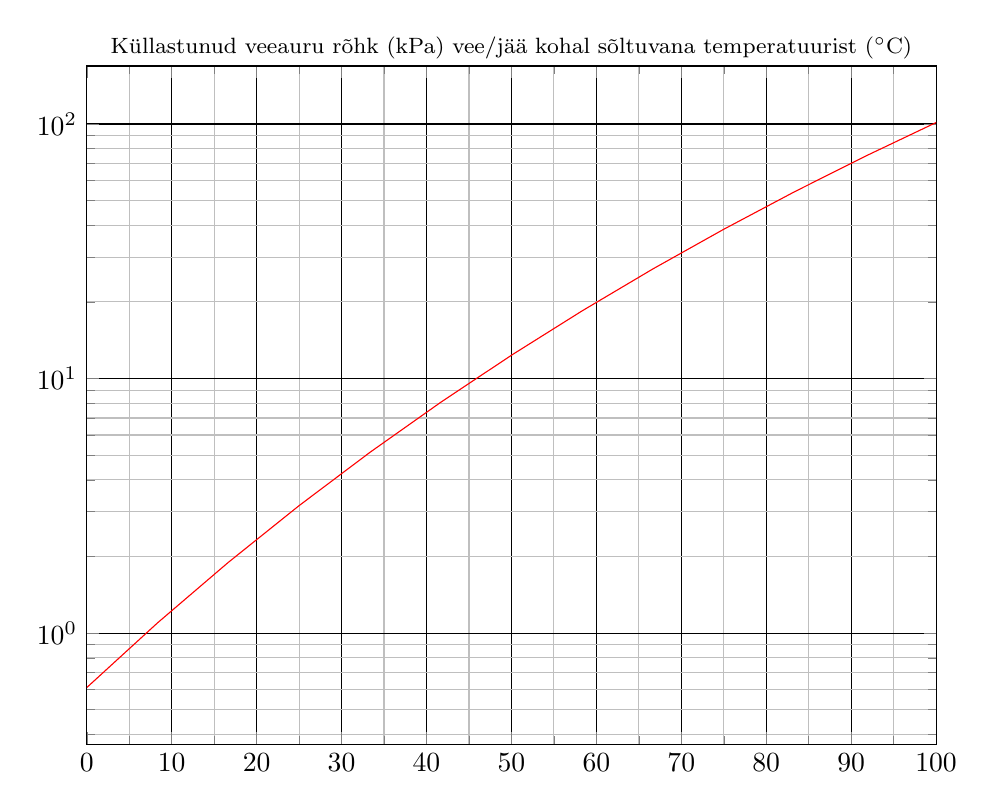
\begin{tikzpicture}
      \begin{axis}[
        ymode=log,
        width=1.02\textwidth,
        height=29em,
        minor tick num=1,
        major grid style = black,
        grid=both,
        % xlabel=$t$ (\unit{\celsius}),
        % ylabel=$P$ (\unit{\kPa}),
        xmin = 0, xmax = 100,
        title={\footnotesize Küllastunud veeauru rõhk (\unit{\kPa}) vee/jää kohal sõltuvana temperatuurist (\unit{\celsius})},
        title style={xshift=0, yshift=-7pt},
        ]
        \addplot[red, domain=0:200] {0.61121*exp((18.678-x/234.5)*(x/(257.14+x)))};
        \addplot[blue, domain=-200:0] {0.61115*exp((23.036-x/333.7)*(x/(279.82+x)))};
      \end{axis}
    \end{tikzpicture}
  }
  \vspace{-1em}
\end{figure}

\yl{PIKNE}
Pikselöögi ajal on keskmine voolutugevus $I=\qty{50}{\kA}$ ning selle löögi kestvus
$\tau=\qty{600}{\us}$. Vaakumi dielektriline läbitavus $\varepsilon_0=\qty{8.85e-12}{\F\per\m}$.\\
\osa Hinnake, millise murdosa oma laengust kaotab äikesepilv, kui elektrivälja tugevus enne pikselööki oli maapinna lähedal $E=\qty{20}{\kV\per\m}$.  Äikesepilve diameeter $d=\qty{24}{\km}$. \emph{Vihje}: võite maapinda vaadelda kui plaatkondensaatori alumist plaati ja äikesepilve kui selle ülemist plaati.\\
\osa Pinnase eritakistus on $\rho = \qty{100}{\ohm\m}$. Inimene seisab äikse ajal paljajalu ja jalad harkis ning saab märkimisväärse elektrilöögi, sest jalgadele rakendub pinge $V=\qty{300}{\V}$. Hinnake, kui kaugele inimesest lõi välk maasse.
\punktid{12} \autor{Jaan Kalda}

\newpage
\yl{PINGPONG}
Juuresoleval graafikul (suuremalt lisalehel) on toodud heli intensiivsus (detsibellides) funktsioonina ajast, kui pingpongipall põrkab üles-alla vastu horisontaalset lauda. Heli tugevuse andmepunktid on võetud ligikaudu iga \num{0.1} sekundi järel. Leidke graafikut kasutades nii täpselt kui võimalik, mitu protsenti palli kineetilisest energiast muundub iga põrke ajal soojuseks\\
\osa esimeste põrgete ja \\
\osa viimaste põrgete jaoks.\\
Pidage silmas, et see protsent püsib enam-vähem konstantne esimesest kuni viienda põrkeni ning samuti alates kolmeteistkümnendast põrkest kuni põrkumiste lõpuni.
\punktid{12} \autor{Jaan Kalda}
\begin{figure}[!h]
  \centering
  \includegraphics[width=\textwidth]{pingpong}
\end{figure}

\end{document}

